\documentclass[12pt,titlepage]{scrreprt}
\usepackage[ngerman]{babel}
\usepackage[utf8]{inputenc}
\usepackage{color}
\usepackage{float}
\usepackage[a4paper,lmargin={2.5cm},rmargin={2.5cm},tmargin={2.5cm},bmargin = {2cm},footskip={1cm}]{geometry}
\usepackage{amssymb}
\usepackage{amsthm}
\usepackage{graphicx}
\usepackage{subfig}
\usepackage{wrapfig}
\usepackage{url}
\usepackage{calc}
\usepackage{overcite} 
\renewcommand\citeform[1]{[#1]}
\usepackage{hyperref}
\hypersetup{
% colorlinks=false,
  pdfborder={0 0 0}
}

\newcommand{\jens}{Prof. Dr. Jens Greinert }
% !TEX program = xelatex
\begin{document}
% % Activate the following line by filling in the right side. If for example the name of the root file is Main.tex, write
% "...root = Main.tex" if the chapter file is in the same directory, and "...root = ../Main.tex" if the chapter is in a subdirectory.
 
%!TEX root =  TNTinderSee.tex

% mehrere Bilder in einer Bildumgebung mit 
%\subfloat{bild.jpg}


\begin{titlepage}
\thispagestyle{empty}
 \begin{center}
 \begin{figure}[htbp]
    \centering
 %   \subfloat{\includegraphics[width=0.15\textwidth]{Bilder/Titel/bild-firma.JPG}}\quad
   %  \subfloat{\includegraphics[width=0.25\textwidth]{Bilder/Titel/bild-uni 
%oder fh.JPG}}
\end{figure}
\vspace*{1cm}
 \Large{Schiller-Gymnasium Offenburg }

  \vspace*{1.5cm}
 {\huge Thema}
 \vspace*{1cm} \\
 {\Large Abschlussbereicht\\von\\Eitel, Martin \\ \texttt{marjelly1@gmail.com}\\Komyakov, Alexander \\\texttt{alexander.komyakov@lynxisgod.eu} \\ Rehwinkel, Antonio \\ \texttt{antonio.rehwinkel@schiller-og.de} \\ Sauerbrey, Luisa \\ \texttt{luisa.sauerbrey@schiller-og.de}
 \vspace{0.5cm}
 {\Large \bfseries \\}
 \vspace{0.5cm}
 {\Large geboren am dein Geburtstag}
 \vfill
  \vspace*{1.5cm}
\begin{table}[h]
	\centering
	\begin{tabular}{|l| l|}\hline
		Aufgabensteller & Prof. \\ \hline
		Durchgeführt bei: & Firmenname\\ \hline
		Betreuer: & Betreuer Firma\\ Marek Czernohous \\ \hline
		Wissenschaftspate & \\ Prof. Dr. Jens Greinert\\ \hline
		Arbeit vorgelegt am: & Datum\\ \hline
	\end{tabular}
\end{table}
}
\end{center}
\end{titlepage}


\begin{titlepage}

	

\title{Die Auswirkung von Munitionshalden auf die Wasserqualität der Ostsee zwischen Vilm und Lauterbach}
\subtitle{Ausfahrt vom 18.07. - 21.07.2021}
\titlehead{\centering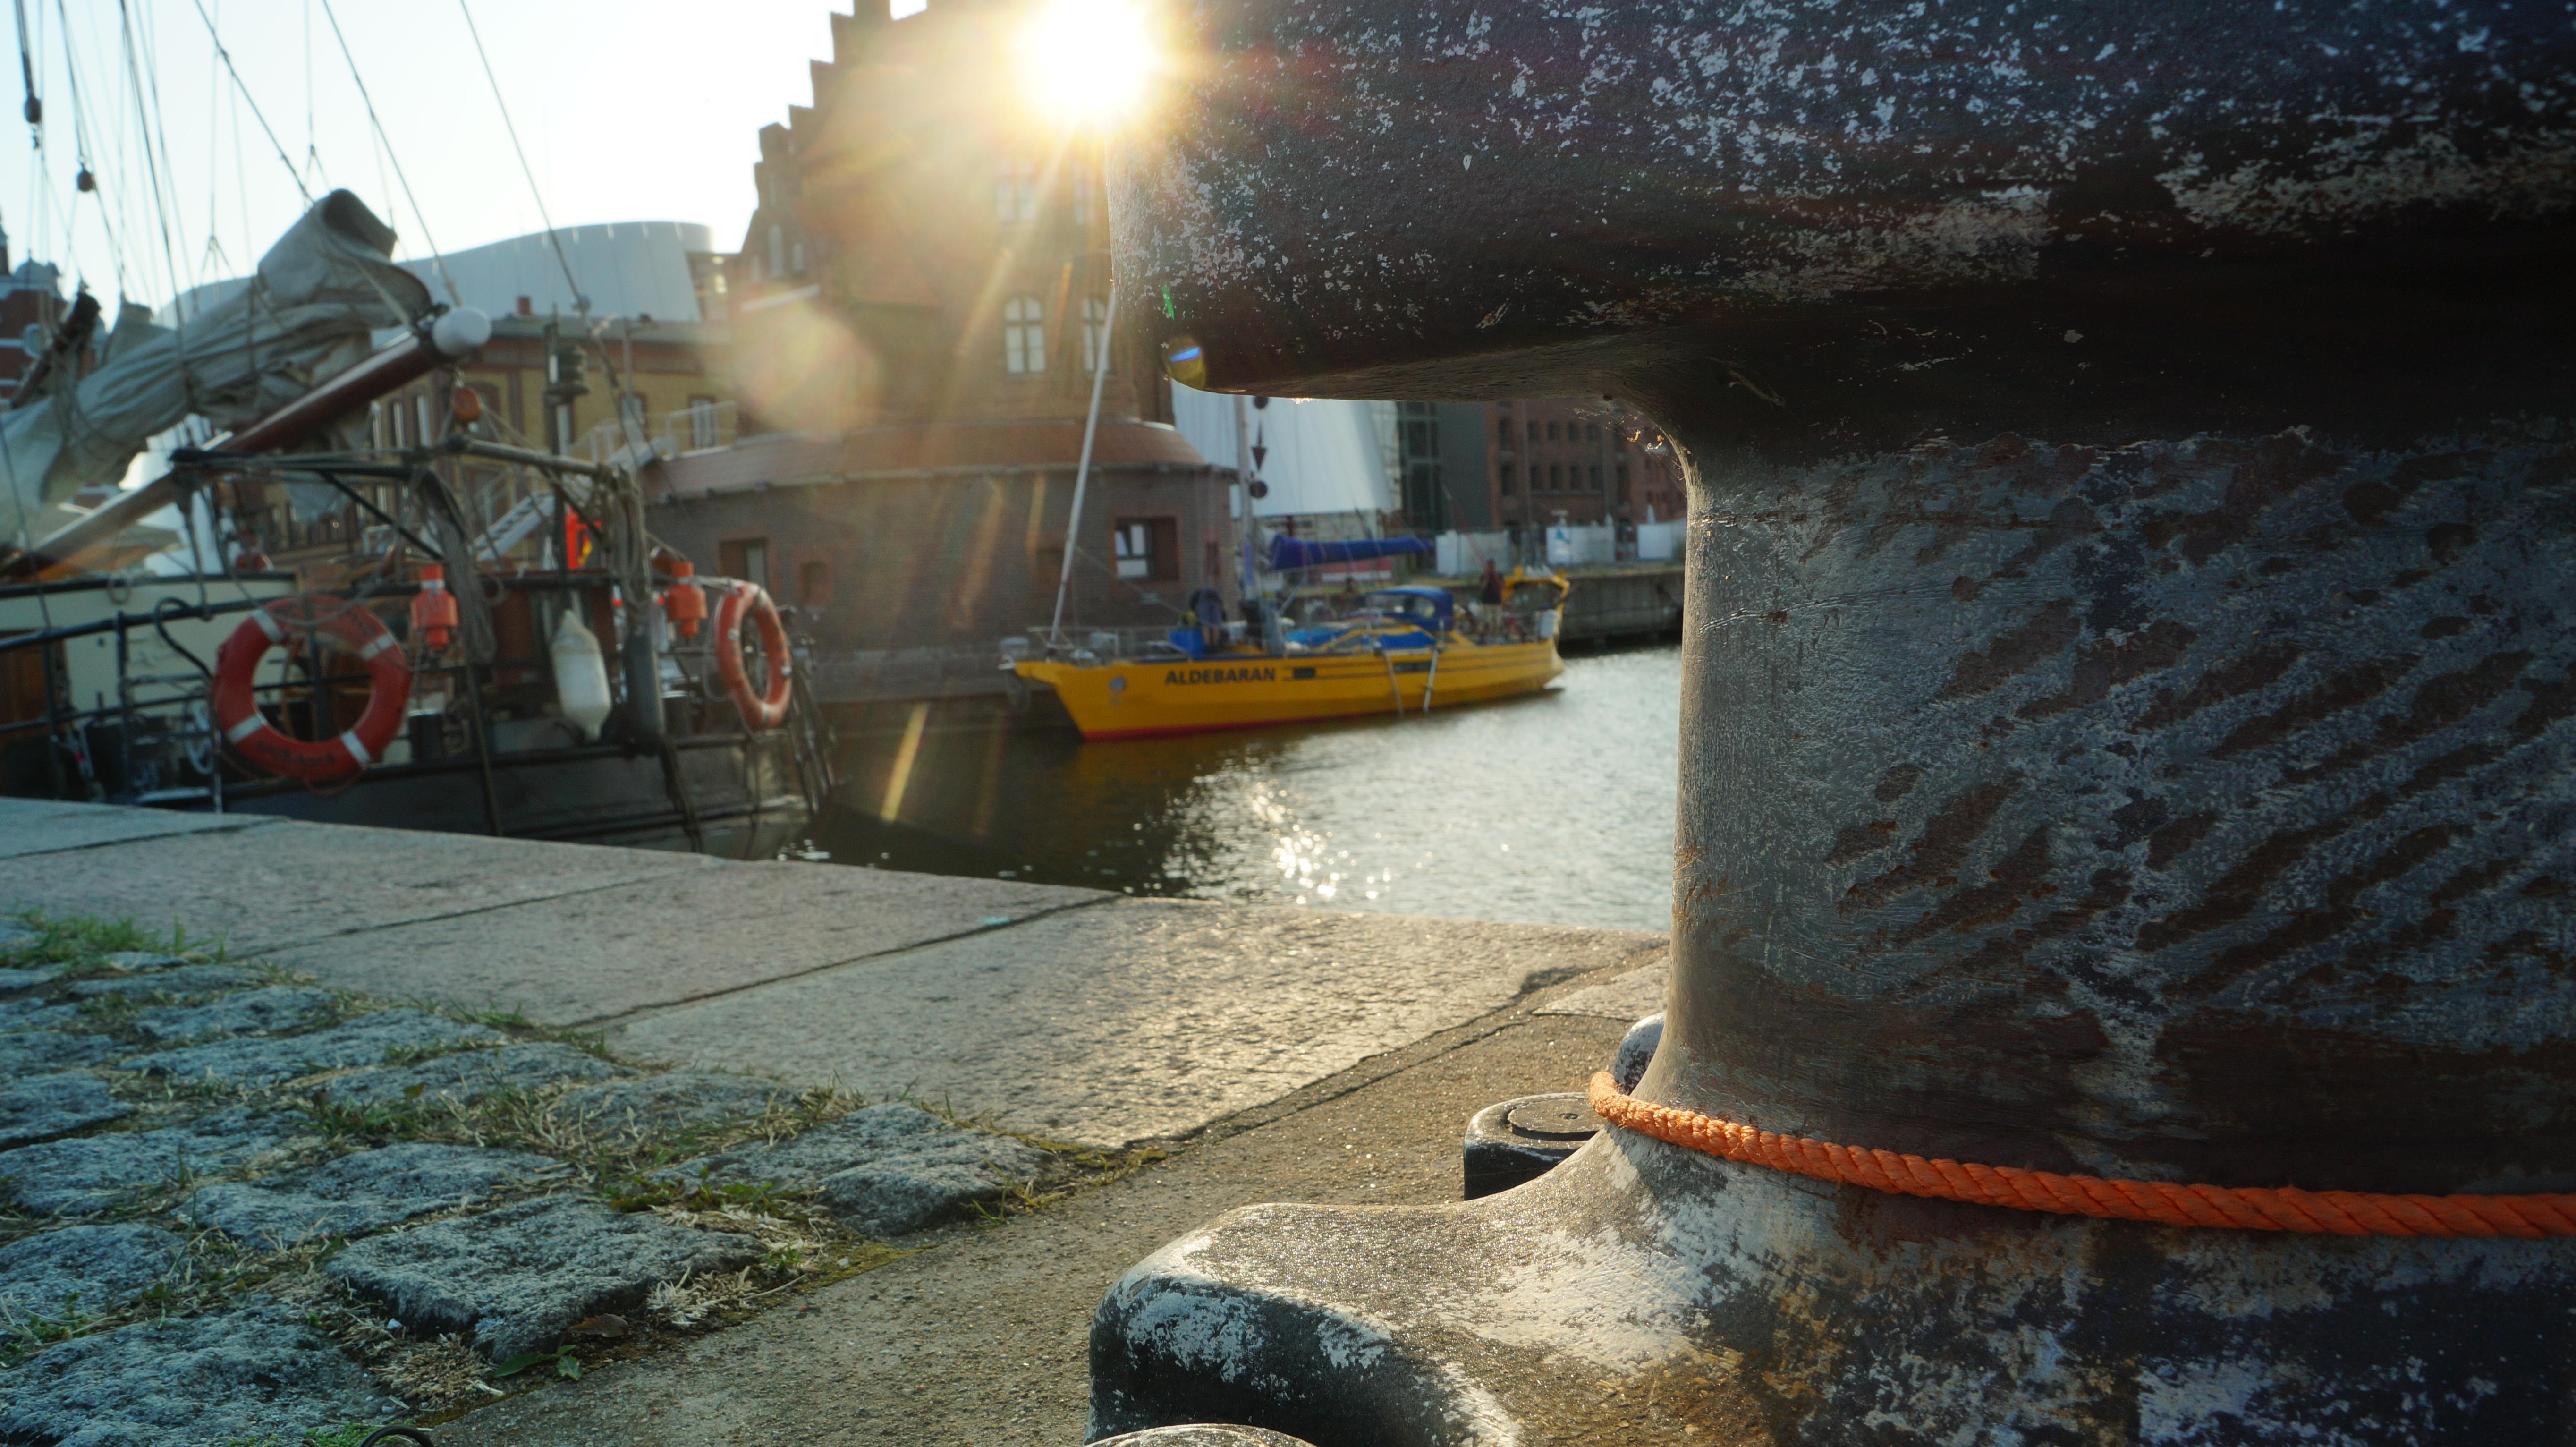
\includegraphics[width=15cm]{Bilder/DSC05220}}


\author{Eitel, Martin; Komyakov, Alexander; \\ Rehwinkel, Antonio; Sauerbrey, Luisa\\ \and Schiller-Gymnasium Offenburg}

\publishers{Wissenschaftspate: \jens \texttt{jgreinert@geomar.de} \\
\vspace*{2ex} Betreuer: Marek Czernohous \texttt{m.czernohous@schiller-offenburg.de}}
%- \\ Schiller-Gymnasium Offenburg}

\maketitle

\end{titlepage}
\addchap{Kurzfassung}
Für unseren Wettbewerbsbeitrag haben wir das Seegebiet zwischen dem Hafen Lauterbach auf Rügen und der Insel Vilm kartiert und beprobt. \\ Das Ziel dabei ist gewesen, etwaige Munitionshalden aufzuspüren 
und mit Gewässer- und Sedimentproben die Umweltbelastung durch sprengstofftypische Verbindungen zu untersuchen.
\\ Die Fragestellung dabei: Wie dringend sollte die Bergung versenkter Munition vor der Südostküste Rügens in die Wege geleitet werden?
Folgende Fragen haben wir uns im Vorfeld gestellt:
\begin{itemize}
\item Besteht vor Ort eine konkrete Gefahr vor allem für Tiere und Mensch durch Altmunition im Meer und ist ein weiteres Monitoring der Gewässer um Rügen erforderlich, um die Gefahren durch versenkte Munition einschätzen zu können? 
\item Wie lassen sich mit einem Multibeam Kartierungen zuverlässig durchführen? Sind neben etwaiger Munitionshalden bspsw. Seegraswiesen zu identifizieren?
\item Lassen sich aus dem Bildmaterial unseres Unterwasserroboters über photogrammetrische Verfahren 3D-Modelle erzeugen?
\end{itemize}
Um diese Fragen zu beantworten, haben wir das anvisierte Gebiet großflächig mit einem Multibeam (vgl: \cite{multib}) kartiert, Wasser- und Sedimentproben genommen und ausgewertet (zum derzeitigen Zeitpunkt mit Ausnahme der Sedimentproben) und auffällige Positionen zur genaueren Begutachtung mit einem ROV angefahren.\\
Für den von uns kartierten Bereich kann in Hinsicht größerer Munitionshalden Entwarnung gegeben werden, mit Multibeam und optischer Erkundung waren keine Auffälligkeiten in Hinsicht sprengstofftypischer Objekte auszumachen. Auch die chemische Analyse der Gewässerproben haben keine Auffälligkeiten gezeigt, so dass davon ausgegangen werden kann, dass es keine außergewöhnlichen Belastungen von sprengstofftypischen Verbindungen auf der Südostseite von Rügen gibt.\\
Mit den Multibeam-Kartierungen konnten in nur kurzer Kampagnenzeit auch bei mobiler Installation auf der Aldebaran großflächige Karten erstellt werden, die deutlich die Ausdehnung von Seegras und Makrophyten zeigen und die in ihrer Abdeckung und Auflösung Kartierungen durch Taucher weit übertreffen. \\
Obwohl wir wegen der mangelnden Kameraqualität unseres ROVs keine 3D-Modelle aus dem Bildmaterial erzeugen konnten, ist die generelle Machbarkeit, bei Installation einer anderen Kamera mit günstigerem Aufnahmewinkel, gegeben.

\tableofcontents
% Activate the following line by filling in the right side. If for example the name of the root file is Main.tex, write
% "...root = Main.tex" if the chapter file is in the same directory, and "...root = ../Main.tex" if the chapter is in a subdirectory.
 
%!TEX root =  TNTinderSee.tex

\chapter[Einleitung]{Einleitung}

Im Meer lagernde Munition stellt eine Gefahr dar. Nicht unbedingt durch unmittelbare Detonotationsgefahr, 
sondern durch die langsame Zersetzung, die die enthaltenen Sprengstoffe nach und nach 
freilegt\cite{zeitbomben}. Die Entstehung sprengstofftypischer Abbauprodukte, sowie das direkte Austreten 
giftiger Stoffe, stellen Gesundheitsgefährung exponierter Meerestiere, aber auch Menschen dar, denn die
Abbauprodukte gelten als krebserregend und das potentiell austretende Phosphor lagert sich an den Stränden 
ab und ist von Bernstein kaum zu unterscheiden. Als wir den Meereswettbewerb mit der Aldebaran fanden, 
fühlten wir uns gezwungen nachzuforschen wie groß die Gefahr schon heutzutage ist.\\

Wir wollten in einem potentiellem Munitionsabwurfsgebiet messen, wie groß die Anteile der Schadstoffe sind und 
ob noch etwas von den Granaten und Bomben zu sehen ist. Dazu entschieden wir uns für ein Gebiet kurz Vilm,
da hier angeblich zwei Schuten nach dem Zweiten Weltkrieg mit Munition beladen explodiert sein sollen.\\

Das Naturschutzgebiet Vilm liegt in etwa 100 Meter Entfernung zu der Explosionsstelle und auch weiter 
entfernte Orte können durch Ablagerungen und Schadstoffe in Fisch-Fängen betroffen sein.\\

In Zusammenarbeit mit der Aldebaran und dem Geomar wollten wir die Wracks kartieren und die Schadstoffwerte in
der direkten Umgebung messen. Besonders interessant wäre die beförderte Munition gewesen. Die Frage der
Ortung und Untersuchung der möglichen Funde konnten wir zusammen mit dem Geomar lösen. Mithilfe eines 
"Multibeams" sollten wir interessante Orte ohne Tauchgang finden können um später mit dem Schuleigenen 
ROV die Orte genauer unter die Lupe nehmen zu können. Auch Sedimentproben dirket neben den Fundstätten 
konnten wir mithilfe eines eignene Aufsatzes realisieren.

Wir befürchteten hohe Werte für Phosphor und sprengstofftypische Verbindungen wie Trinitrotoluol (TNT) 
zu messen und unter Umständen sogar Granaten oder Bomben zu finden. Falls dies passieren sollte, würde 
sich für uns die Frage stellen, wie sich diese Munition auf die Öknomie ausgewirkt hat. 

Themenfindung, Relevanz, entscheidende Fragen, Lösungsansätze, Forschungsstand mit Quellen, Erwartungen, konkrete Fragen.

\chapter{Hauptteil}
\section{Versuchsplanung}
Um unsere Forschungsfragen beantworten zu können, haben wir uns für vier verschiedene Mess- und Beprobungsarten entschieden. Die Kartierung mit einem Multibeam, die Wasserprobenentnahme mit einem Wassersampler, die Sedimententnahme mit unserem ROV und einer Probenschaufel und der optischen Erkundung auffälliger Orte am Meeresboden mit der Kamera unseres ROVs.
\subsection{Kartierung}
\subsubsection*{QGIS}
Die Kartierungsvorgänge wurden alle mit der Free Open Source Software \emph{QGIS}\cite{qgis} durchgeführt.
\begin{figure}[ht]
    \centering
    \includegraphics[width=6cm]{QGIS/about-screenshot.png}
    \caption[fig:qgisabout]{QGIS-Benutzeroberfläche}
\end{figure}
\\Mithilfe dieser Software lassen sich basierend auf bereits existierenden Karten, 
wie beispielsweise OpenStreetMap\cite{ostrm} oder OpenSeaMap\cite{oseam}, eigene Routen sowie
Points of Interest(POIs) ohne großen Aufwand eintragen. Genauso leicht erfolgt der Import der von 
Navigationsgeräten der ALDEBARAN gespeicherten Routen. 

\subsection{Wasserproben}
% Activate the following line by filling in the right side. If for example the name of the root file is Main.tex, write
% "...root = Main.tex" if the chapter file is in the same directory, and "...root = ../Main.tex" if the chapter is in a subdirectory.
 
%!TEX root =  TNTinderSee.tex

Das Multibeam erledigte einen großen Teil unserer Arbeit, doch trotzdem stellten wir uns die Frage was wohl wäre, wenn sich noch Bomben oder ähnliches auf dem Meeresboden befinden, wir allerdings an dieser Stelle zufällig genau nicht vermessen. Mithilfe von Jens Greinert kamen wir dann auf die Idee, an bestimmten Punkten auf unserer Strecke Wasserproben zu nehmen. 

Der Vorteil der Wasserproben war natürlich, dass sich nicht genau an der Stelle wo wir sie entnommen hatten eine Bombe hätte sein müssen, sondern es reichte wenn sich Sprengstoffähnliche Verbindungen im Wasser befinden, vielleicht auch von weiter weg.  

\subsubsection{Technische Beschreibung und Durchführung an Board}
Die Wasserproben waren relativ simpel aufgebaut. Wir hatten ein Plastikrohr mit Deckeln, welche mithilfe von zwei Gummis offen gehalten wurden. Das Rohr wurde ins Wasser gelassen, jeweils abgestimmt auf die Tiefe etwa einen Meter oben dran, sodass aufgewirbelter Dreck oder Algen nicht im Weg waren. Sobald es sich an der richtigen Stelle befand, wurde ein kleines metallenes \emph{Engelchen} dem Seil an welchem das Rohr war entlang, in die Tiefe geschickt. Das Engelchen war aufgrund von seinem Material relativ schwer, wodurch sich die Gummis an dem Rohr lösten und die Deckel zu gingen. Danach musste die Probe nur noch hoch gezogen werden.

Sobald sich die Probe wieder auf dem Boot befand konnten wir weiter fahren zu dem nächsten Standpunkt wo eine hohe Wahrscheinlichkeit bestand etwas zu finden. Auf dem Boot ging dann allerdings erst die richtige Arbeit los, nämlich aus der rohen Wasserprobe eine zu machen, aus welcher man auch Informationen ziehen konnte. An dem Rohr befand sich ein kleines Ventil, wodurch wir das Wasser langsam und kontrolliert in einen Messbecher laufen lassen konnten. Mit viel Feingefühl versuchten wir genau 1000ml zu bekommen. Es würde keinen großen Unterschied machen, wenn es mehr oder weniger wäre, allerdings hat uns das einiges an Rechnen erspart. 

Das abgemessene Wasser wurde anschliessend durch einen selbst gebauten Trichter in ein \emph{Blood Bag} gefüllt, solche wie man auch in Operationen finden würde, um normalerweise Blut zu lagern. In unserem Fall war dies allerdings nur ein Zwischenschritt. 
An dem dem Blood Bag befestigten wir einen kleinen Schlauch befestigtenmit einem Filter, durch das das Wasser gelassen wurde. Im Anschluss an den Filter, welcher lediglich Schmutzpartikel aus dem Wasser filterte, befand sich ein kleines Teströhrchen mit einer Art Granulat. Dieses war nach unten hin offen, da das fertig durchgelaufene Wasser unbrauchbar für uns war, weshalb wir es einfach langsam abtropfen lassen konnten.

Die eigentliche Magie war nun das geschehen in dem Granulat. Dieses war nämlich absichtlich dafür, um schadstoffähnliche Verbindungen aus dem Wasser zu filtern und zu speichern. Dazu kam noch die Anforderung, dass man möglichst genau einen Liter durch das Teströhrchen laufen lassen sollte, um einen möglihst genauen Vergleich ziehen zu können, wo sich eventuell mehr oder weniger Verbindungen befanden. Natürlich ist es auch möglich anhand von anderen Stoffen im Wasser zu bestimmen, wie viel Milliliter Wasser man genau benutzt hat, doch für uns war es so am einfachsten. 

\subsubsection{Probenpräparation am GEOMAR}
Die Teströhrchen haben wir anschließend mit ins Geomar nach Kiel genommen. Dort haben wir die Proben für den Ionenchromatographen präpariert, indem eine definierte Menge von destilliertem Wasser über das Granulat haben laufen lassen. Anschließend wurden die Proben mit einem Verdünnungsmittel auf 2ml aufgefüllt. Diese nun fertige Probe wurde dann auf Rückstände sprengstofftypischer Verbindungen analysiert.
\begin{figure}[]
    \centering
    \includegraphics[width=0.8\linewidth]{Bilder/DSC05766-scaled.jpg}
    \caption{Vorbereitung der Wasserproben für den Ionenaustauschchromatographen}
    \label{fig:praep}
\end{figure}
\subsection{Sedimentproben}
% Activate the following line by filling in the right side. If for example the name of the root file is Main.tex, write
% "...root = Main.tex" if the chapter file is in the same directory, and "...root = ../Main.tex" if the chapter is in a subdirectory.
 
%!TEX root =  TNTinderSee.tex

Sedimentproben haben wir an den Stellen entnommen, an denen ungewöhnliche Erhebungen am Meeresboden zu finden waren. 
Dazu sind wir mit dem ROV bis auf den Meeresboden gefahren um mit der Probenschaufel dort von der Bodenoberfläche eine Bodenprobe an die Oberfläche zu bringen. Dort wurde die Probe in einem Probenbeutel zur späteren Analyse gesichert.


\subsection{Multibeamparametermessungen}
% Activate the following line by filling in the right side. If for example the name of the root file is Main.tex, write
% "...root = Main.tex" if the chapter file is in the same directory, and "...root = ../Main.tex" if the chapter is in a subdirectory.
 
%!TEX root =  TNTinderSee.tex

Da das vollständige Abfahren des Gebiets mithilfe des ROVs nicht möglich gewesen wäre, 
brachten die Forscher des Geomar ein Multibeam mit auf die Aldebaran. \\
Ein Multibeam funktioniert ähnlich wie ein Echolot, es sendet eine Schallwelle in die zu messende 
Richtung und wartet darauf dieses Signal wieder zurückzubekommen. Durch den Zeitunterschied 
kann die Entfernung bestimmt werden. Der größte Unterschied zwischen einem Echolot und dem Multibeam 
liegt hierbei bei der Anzahl der "Beams". \\
Das von uns verwendete Multibeam kann mit 512 Einzel-Echoloten großflächig den Meeresboden kartieren. 

\subsection{ROV-Untersuchung}

Unsere Grundlegende Idee zur ROV Analyse war vollgende, erst wollten wir das als Munitionsbelastete gekennzeichnete Gebiet mithilfe 
des Multibeams grob Katieren und nach genauere Betrachtung 
Interessante bzw. auffällige Stellen finden. Daraufhin wollten wir diese mit unserem ROV antauchen um diese genauer Bestimmen zu können.
Dieses Vorgehen konnten wir auch so zum großteil durchführen.
Die genauer zu bestimmenden Stellen haben wir mit unserem eigenen ROV (Remotely Operated Vehicle) eine Art Tauchroboter angetaucht. 
Dieser entstand vor 3 Jahren in unsere Forschungsgruppe aus einem Bausatz der Firma BlueRobotics und trägt die Bezeichnung "Blue ROV 2".
Der Tauchrobter lässt sich mithilfe eines Laptops und eines Controllers über ein langes Kabel (auch Tether genannt) frei in alle Richtugen in der Wassersäule bewegen.
Und zusammen mit der schwenkbare live Kamera war unser ROV das Perfekte Inspektionsfahrzeug für unsere Forschungziel. Der ROV wird optimaler weise 
von vier Personen bedient da zwei Personen die Tetherspule bedienen müssen, man einen Navigator benötigt, da die Orientierung Unterwasser in einem fremdem Gebiet sehr anspruchsvoll Inspektionsfahrzeug und das ROV von einem Piloten Gesteuert werden muss.
Somit beansprucht das ROV fahren unser gesamtes Forschungsteam und die Restlich Crew um das Boot auf position zu Halten, wodurch das ROV fahren nicht nur einen hohen zeitlichen aufwand hat, sondern auch die gesamte Kapazität der Crew benötigt.
Aus diesem Grund war es noch viel wichtiger geziehlte Stellen ausfindig zu machen an denen wir mit dem ROV abtauchen wollten und nicht nur blind im Meeresboden rumstochern.
\\

Das ROV von BLueRobotics besteht aus zwei runden Druckgehäusen eine für den Lithium-Ionen Akku, die andere für die Steuerungselektonik und die Kamera.
Vor jedem Tauchgang müssen diese Druckgehäuse mithilfe einer Vakumpumpe auf ihre dichtigkeit überprüft werden. 
Daraufhin kann das ROV mithilfe des Tethers an den Laptop angeschlossen werden, auf dem sich die Steuerungssoftware befindet.
Um die Abläufe des ROV tauchens einzuspielen und den ROV auf der Aldebaran zu testen haben wir am Sonntag Abend einen Testtauchgung im Hafen durchgeführt. 
Hierbei ist uns schon die Schlechte Sicht in der Ostee aufgefallen, die uns später noch einige Schwierigkeiten machen sollte.
\\

Insgesamt haben wir für unsere Forschung auf der Aldebaran an drei Unterschiedlichen Stellen Insgesamt Fünf ROV Tauchgänge durchgeführt 
%Einfügen Karte mit Tauchstellen des ROV mit Objekten auf dem Multibeam
Während diesen Tauchgängen und bei deren Vorbereitung hatten wir mehrere Schwierigkeiten die aufgrund unserer Begrenzten Zeit und Kapazität unsere Forschung verkompliziert hat.
Da die Aldebaran ein verhältnissmäßig kleines Schiff für ein Forschungsschiff ist, hat sie zwar den Vorteil dass sie gerade durch das einklappbares SChwert einen sehr geringen Tiefgang von 80 cm hat, was uns die Forschung in diesem Gebiet erst ermöglicht hat.
Anderrerseits ist sie deshalb auch sehr Anfällig gegenüber Wind und Wetter, weshalb das Arbeiten an Deck bei den Zeitweise aufgetretenen Windstärken von vier bis fünf erschwert wurde.
Dies hat sich sowohl bei der Vorbereitung des ROVs gezeigt als auch bei den Tauchgängen, da die Aldebaran trotz Anker hin und her pendelte, wodurch sich die Position ständig verändert hat.
Die Navigation und die Orientierung Unterwasser mit dem ROV war mit Abstand die größte herausforderung, da die einzige möglichkeit sich zu Orientieren der eingebauter Kompass ist.
Und der ROV aufgrund seiner Größe kein USBL (Ultra Short Baseline) - System besitzt, wodurch die genaue Position des ROVs nicht bekannnt ist.
Deshalb ist die einzige möglichkeit eine genaue position, dort wo das auffälige Objekt durch das Multibeam ausgemacht wurde, anzutauchen, indem man durch die Bekannte Position des Schiffes und somit den Startpunktes des ROVS, das Objekt anpeilt und den ROV genau auf diesem Kompasskurs hält.
Was hierbei nicht ganz trevial war dass das Schiff durch das Pendeln stänfig seine Position veränderte.
Den ROV auf einem genauen Kurs zu halten war hierbei problematisch, da durch die geringe Tauchtiefe von ca. 5m das ROV von den Wellen und dem Sturm hin und her geworfen wurde und abgedriftet ist.
Was zusätzlich noch schwierigkeiten bereitet hat war die empfindliche Steuerung, mit der es kompliziert war den ROV auf einer geraden Linie zu halten.
Die interessanten Objekte haben wir mithilfe der optischen Kamera untersucht, jedoch durch die sehr geringe Sichweite in der Ostesee wurde dies sehr erschwert, da man an den Grund bzw. an das Objekt bis auf eine nähe von ca. 20 cm herantauchen musste um das Objekt zu Identifizieren. 
% Activate the following line by filling in the right side. If for example the name of the root file is Main.tex, write
% "...root = Main.tex" if the chapter file is in the same directory, and "...root = ../Main.tex" if the chapter is in a subdirectory.
 
%!TEX root = TNTinderSee.tex 
%%%%%%%%%%%%%%%%%%%%%%%%%%%%%%% 80-Char line %%%%%%%%%%%%%%%%%%%%%%%%%%%%%%%%%%

\chapter{Ergebnisse}
\section{Optische Auswertung der ROV-Bilder}
\subsection{Identifikation von Munition}
Für Hauptteil unserer Forschung, welche sich mit der Suche nach ehemaliger Kriegsmunition und der daraus folgende Umweltbelastung durch sprengstofftypischen Verbindungen beschäftigt,
hatte das ROV die Aufgabe die im Untersuchungsgebiet vermuteten Munitionsreste zu verifizieren. 
Im Jahre 1945 soll der Fißnowkahn Nr. 139 , unter aufsicht des Russischen Militärs ca. 90 Tonnen Kriegsmunition zu versenken sollte, hierbei versenkte sich der Kahn tragischer weise selber und die zu entladende Munition gerieht unkontrolliert in das Gewäßer vor der Insel Vilm.
Mithilfe des Multibeams haben wir vor Vilm zwei kleinere auffälige Objekte entdeckt, welche wir durch den ROV genauer betrachten konnten. Die aufälligere Stelle bestand auf dem Multibeam aus einem ca. 4m langen Objekt mit einem Durchmesser von einem Meter, was von der Größe eine Grundmine hätte sein können.
Nach der Inspektion durch den ROV hat sich zum Glück herausgestellt, das sich das Objekt nur um eine, vermutlich durch ein Anker entstandenr, Rille mit einem Stahlseil darin handelt, und somit keine Gefahr davon ausgeht.
An der zweiten auffälligen Stelle haben wir beim tauchen mit dem ROV nichts finden könne, was einerseits an einer Anomalie des Multibeams liegen könnte und an diesem Ort nichts zu finden war, oder daran dass wir an dem Objekt vorbeigetaucht sind was durch die sehr Schlechte Sicht und den Navigationsschwierigkeiten des ROV ebenfalls eine möglichkeit ist.
Um die von dem ROV gefundenen Objekten einordnen und diese für die Öffentlichkeit besser darstellen zu können wollten wir die Videoaufnahmen der Internen Kamera in einzelne Bildere aufspalten und mithilfe der Software Metashape durch Photogrammetrie daraus ein 3D-Model erstellen. 
Nach dem extrahieren der einzelnen Bilder und dem impotiern in Metashape hatte das Programm probleme die Einzelnen Kameraperspektiven zu berechnen, trotz einiger tricks und optimierung der Photogrammetrie Daten zusammen mit Yifan Song, einem Spezialisten für Photogrammetrie aus dem Geomar, konnte Metashape kein Fehlerfreies 3D-Model erstellen.
In der Anschließenden Disskusion mit Yifan Song kamen wir darauf dass Metashape aufgrund des hohen Motion Blurs der Kamera und der schlechten Perspektive probleme hatte. 
Als Optimierung für unsere nächste Photogrammetrie mit dem ROV haben wir beschlossen, dass wir eine extra Kamera mit einer höheren Bildfrequenz verbauen werden, um den Motion Blur zu reduzieren, welche senkrecht auf den Boden und auf das Objekt gerichtet ist, so dass die einzelnen Bilder eine höhere Überlappung mit auffälligen Bildpunkten haben.
\\

Der zweite Teil der Vorschung bestand darin herauszufinden, ob man mithilfe des Multibeams Seegraswiesen und Makrophyten Kartieren kann. Hierbei haben wir die Strukturen in der Multibeamkarte mit dem wahren untergrund durch das ROV bestimmt.
Bei der Rückstrahlung der Hydroakustischen Wellen und somit der Struktur der Multibeamkarte spielt einerseits die Flora des Untergrunds eine Rolle, andererseits auch die Art des Sediments.
Aus diesem Grund haben wir einen eigenen Aufsatz für das ROV entwickelt und mit dem 3D-Drucker gedruckt der es uns erlaubt gezielt Sedimentproben zu nehmen, und nach der Analyse der Korngröße auf das Rückstrahlvehalten schließen zu können.
Hierbei ist uns aufgefallen das in der nähe der Seegraßwiesen und Makrophyten das Sediment tendenziell feiner ist und in den Arealen ohne dieser Flora eher gröber.
Um den genauen Verlauf der Flora hin zu den Seegraswiesen mit der Multibeamkarte vergleichen zu können wollten wir ebenfalls ein 3D-Modell erstellen, hierbei hatten wir jedoch die Gleichen Probleme wie bei der Photogrammertrie der aufälligen Objekte, wodurch wir dies leider nicht erstellen konnten.

\section{Wasseranalyse}
\begin{figure}[htb]
\includegraphics[height=\textheight,%
                   width=\textwidth,%
                   keepaspectratio]{Bilder/TIC_3227_SampleW1.PNG}
\caption{Total Ion Count W01 vom 19.07.2021}
\end{figure}
\begin{figure}[htb]
\includegraphics[height=\textheight,%
                   width=\textwidth,%
                   keepaspectratio]{Bilder/TIC_5ppbSTandard.PNG}
\caption{Total Ion Count - Referenzstandard}
\end{figure}
\begin{figure}[htb]
\includegraphics[height=\textheight,%
                   width=\textwidth,%
                   keepaspectratio]{Bilder/Explosives_3227_SampleW1.PNG}
\caption{Chromatografieergebnis mit Focus auf sprengstofftypische Verbindung. Von oben nach unten: HMX (schwarz), RDX (grün), TNT (blau), ADNT (gelb)}
\end{figure}
Es gibt zwei Spitzen für 4-ADNT und 2-ADNT-Isomere.
Was bedeuten die Spitzen bei HMX und RDX?

\begin{figure}[htb]
\includegraphics[height=\textheight,%
                   width=\textwidth,%
                   keepaspectratio]{Bilder/Explosives_5ppb.PNG}
\caption{Vergleichende Standardwerte}
\end{figure}
\begin{figure}[htb]
\includegraphics[height=\textheight,%
                   width=\textwidth,%
                   keepaspectratio]{Bilder/MC_data_Aldebaran.pdf}
\caption{Datensatz}
\end{figure}
\section{Diskussion der Ergebnisse}
Wir können Entwarnung geben: Das von uns abgesuchte Gebiet ist unbelastet. Ein
solches Ergebnis ist zwar unspektakulär, jedoch auch erleichternd. Wieso 
unsere Proben keine Spuren von Sprengstoffen oder deren Zerfallsprodukten 
enthalten ist eine andere Frage, möglicherweise wurden sie seit dem xx.xx.xxxx%TODO: DATUM
von der Biomasse vor Ort aufgenommen, und uns bei der Probenfiltrierung
abhanden gekommen. Auf jeden Fall sollten weitere Untersuchungen (vorzugsweise
an Bord der ALDEBARAN) stattfinden, sowie evtl. neue Methoden zur Erfassung
von Sprengstoffen in Organik entwickelt werden.


%!TEX root = TNTinderSee.tex 

\chapter[Fazit]{Fazit}

Obwohl unser Untersuchungsgebiet in einem auf Seekarten als \emph{munitionsbelastetem Gebiet} lag, haben wir trotz aufwändiger Kartierung keine Munition gefunden. Zusätzlich haben uns unsere Wasserproben keinerlei Hinweise sprengstofftypischen Verbindungen, wie man sie in der Nähe von vor-sich-hin rostender Munition erwartet, gezeigt. Betrachtet man die Ergebnisse, wäre die gute Nachricht, dass nicht nur das Gewässer südöstlich von Rügen diesbezüglich unbelastet ist und auch von eventuell nicht aufgespürte Munitionsreste keine Gefahr für das Untersuchungsgebiet zu sein scheint. \\
Andere Untersuchungen kommen allerdings zu anderen Schlüssen, so gilt die Munitionshalde \emph{Kohlberger Heide} in der Kieler Bucht als hochbelastet\cite{kohl} \\
Letztendlich sind unsere Ergebnisse deshalb mit Vorsicht zu interpretieren. \\
Eine plausible Erklärung für unsere Ergebnisse wäre, dass die Reste des o.g. Schutenunglücks zu DDR-Zeiten wieder geborgen wurden und wir deshalb am Ort des Unglücks keine Überreste der Schuten oder der Munition mehr gefunden haben.
Zusätzlich könnte die durch das Flachwasser großzügig vorhandene Biomasse eventuelle Restbelastungen aufgenommen haben. Diese spielt in der Ionenchromatografie wegen der notwendigen Filtrierung der Proben nämlich keine Rolle. \\
Um das zu prüfen, müsste die Biomasse gezielt untersucht werden.\\
Vielleicht waren wir aber auch einfach zu weit weg von der nächsten Munitionshalde.\\
\begin{figure}[htb!]
\includegraphics[height=\textheight,%
                   width=\textwidth,%
                   keepaspectratio]{Bilder/karte_muni.PDF}
\caption{Karte der Munitionslagerstätten in Nord- und Ostsee\cite{shmuni}.}
\end{figure}

Trotz unserer Untersuchungsergebnisse bleibt die Gefahr durch Altmunition in der Ostsee weiter bestehen (siehe Abb 4.1.) und es muss dringend ein Konzept zur Bergung und Entsorgung der Munition her, um das Ökosystem Ostsee zu schützen.\\

Diese Forschungsreise war für uns alle eine wunderbare und sicherlich prägende Erfahrung, dafür möchten wir uns bei allen Beteiligten herzlich bedanken.\\

Und falls bei der nächsten Forschungsfrage ein kleiner Tauchroboter inklusive Minicrew benötigt werden sollte: Wir denken, die See schuldet uns noch was. :-)





% Activate the following line by filling in the right side. If for example the name of the root file is Main.tex, write
% "...root = Main.tex" if the chapter file is in the same directory, and "...root = ../Main.tex" if the chapter is in a subdirectory.
 
%!TEX root =  TNTinderSee.tex

\chapter[Danksagungen]{Danksagungen}
Wir danken Prof Dr. Jens Greinert vom GEOMAR Kiel und Leiter der Arbeitsgruppe DeepSea-Monitoring. Er ist der beste Wissenschaftspate, den wir uns hätten wünschen können.\\
Frank Schweikert und Dr. Hannes Imhof, für die tollen Tage und all die Hilfe an Board der Aldebaran. \\

Mareike Kampmeier für die geduldige Einführung am Multibeam und die vielen Erklärungen zum Thema Sprengstoffe im Wasser. \\

Dr. Inken Suck, die bestimmt coolste ROV-Pilotin



Frank Schweikert und Dr. Hannes Imhof von der deutschen Meeresstiftung, für die tollen Tage und all die Hilfe an Board der Aldebaran. \\


Mareike Kampmeier vom GEOMAR Kiel für die geduldige Einführung am Multibeam und die vielen Erklärungen zum Thema Sprengstoffe im Wasser. \\


Dr. rer. nat. Inken Suck vom GEOMAR Kiel, der bestimmt coolsten ROV-Piloten dafür, dass sie uns gezeigt hat, wie man Unterwasserfahrzeuge richtig navigiert. \\


Maria Martinez Cabanas vom GEOMAR Kiel dafür, dass sie uns und unsere Proben in Ihre Labore mitgenommen hat, und geduldig stundenlang alle Fragen beantwortet hat.\\


Dr. Kevin Köser vom GEOMAR Kiel für den inspirierenden Vortrag über Photogrammetrie \\


Yifan Song vom GEOMAR Kiel dafür, dass er uns ganz praktisch beigebracht hat, wie man Videomaterial georeferenziert.\\


Marek Czernohous für die insgesamt über 24 Stunden Fahrzeit, die Mate, Franzbrötchen und enorme Hilfe beim \LaTeX -Satz.\\



\bibliography{bibliography}
\bibliographystyle{plain}
\include{Anhang}
\end{document}
